% ------------------------------------------------------------
% File: figures/fig-iteration-2-recess-comparison.tex
% Iteration 1 to Iteration 2 recess microscopy comparison
% ------------------------------------------------------------

\begin{figure}[htbp]
  \centering
  \begin{tikzpicture}[
    font=\footnotesize,
    imglabel/.style={draw, fill=white, line width=0.35pt, inner xsep=4pt,
      inner ysep=2pt, font=\small\bfseries}
  ]
    \node[anchor=north west, inner sep=0pt] (oldRecess) at (0,0) {
      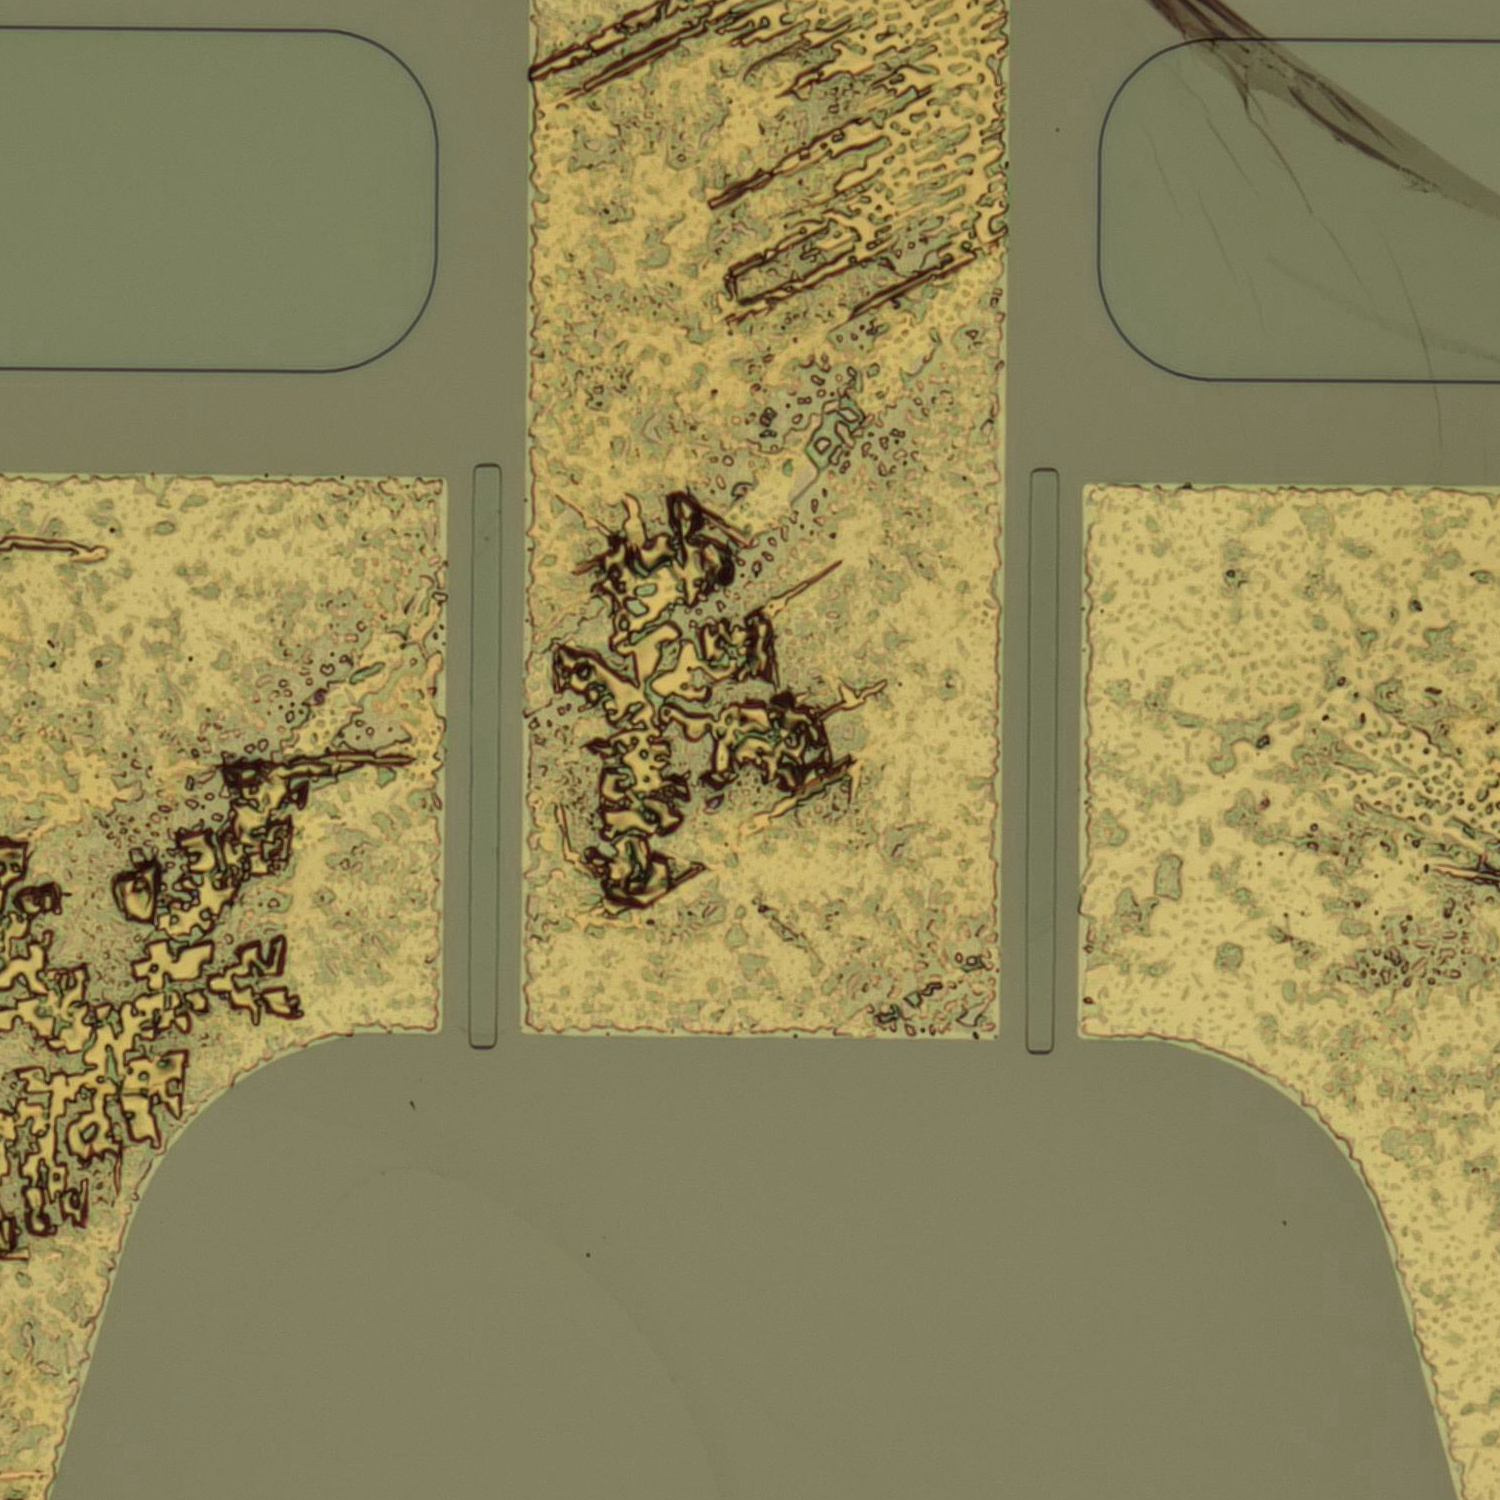
\includegraphics[width=0.38\linewidth]{figures/fabrication_images/enhancement_mode_images/iteration2/old_recess.jpg}
    };

    \node[anchor=north west, inner sep=0pt] (newRecess) at ($(oldRecess.north east)+(0.06\linewidth,0)$) {
      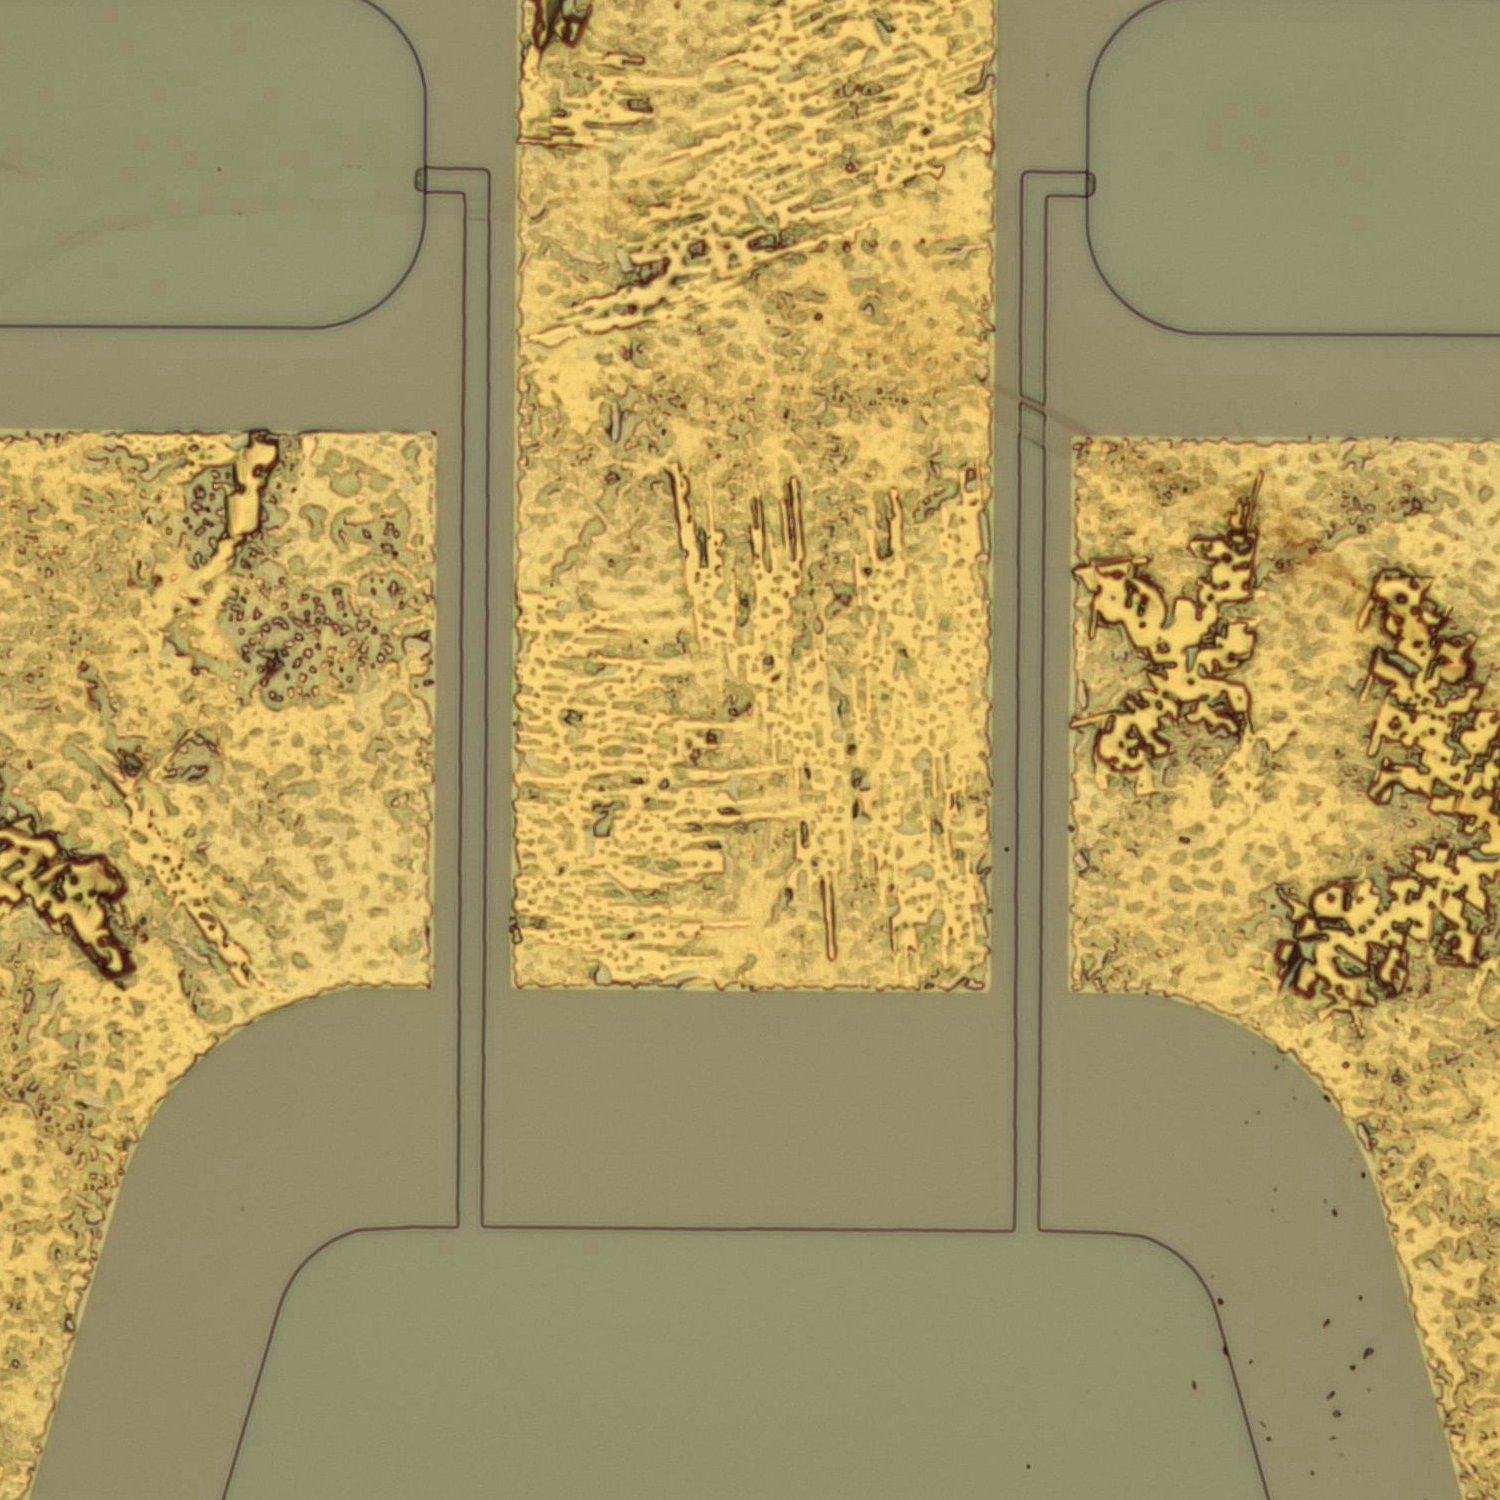
\includegraphics[width=0.38\linewidth]{figures/fabrication_images/enhancement_mode_images/iteration2/etch_gate-1.jpg}
    };

    \node[imglabel, anchor=north, yshift=-1.5mm] at (oldRecess.south)
      {Iteration 1 Recess};
    \node[imglabel, anchor=north, yshift=-1.5mm] at (newRecess.south)
      {Iteration 2 Recess};
  \end{tikzpicture}

  \vspace{2mm}
  \caption{Optical microscopy comparison of the etched recess in
  Iteration 1 and Iteration 2. The revised structure replaced the local
  trench recess with a larger recessed region covering the full gate region.}
  \label{fig:iteration2-recess-comparison}
\end{figure}
